\subsubsection{Genetischer Algorithmus}
\label{sec:Description_GenetischerAlgorithmus}

\minipagedOrBelowEachOther
{
    \paragraph{Idee}
    Der genetische Algorithmus (\gls{GA}) \cite{mirjalili2018genetic} ist ein evolutionärer Optimierungsalgorithmus, der von den Prinzipien der natürlichen Selektion und 
    Genetik inspiriert ist. Er wird verwendet, um optimale oder nahezu optimale Lösungen für komplexe Probleme zu finden, 
    indem er eine Population von möglichen Lösungen (Individuen) iterativ verbessert.

    Ein Individuum setzt sich aus einer Menge von Genen zusammen, die zusammen ein Chromosom bilden.
    Die Gene repräsentieren die Parameter oder Variablen des zu optimierenden Problems.
    \vspace{1cm}

    \paragraph{Grundprinzip}
    Der Algorithmus beginnt mit einer zufällig generierten Population von Individuen.
    Die Anzahl der Individuen in der Population wird durch die Populationsgrösse $N$ bestimmt und 
    bleibt während des gesamten Optimierungsprozesses konstant.
    Jedes Individuum $\overrightarrow{I_{\mathbf{i}}}$ wird anhand einer \gls{Fitnessfunktion} bewertet, die misst, 
    wie gut es das Optimierungsziel erfüllt.
    Basierend auf den \gls{Fitness}werten werden Individuen ausgewählt, um sich zu paaren und Nachkommen zu erzeugen.
    Die Paarung erfolgt durch genetische Operationen wie Kreuzung (Crossover) und Mutation.
    Die Kreuzung kombiniert die Gene zweier Elternindividuen, um neue Nachkommen zu erzeugen, 
    während die Mutation zufällige Änderungen an den Genen eines Individuums vornimmt, um genetische Vielfalt zu gewährleisten.
    Nach der Erzeugung einer neuen Generation von Individuen wird die Fitness jedes Nachkommens bewertet.
    Der Prozess der Bewertung, Auswahl, Kreuzung und Mutation wird über mehrere Generationen hinweg wiederholt,
    bis eine Abbruchbedingung erfüllt ist, wie z.B. eine maximale Anzahl von Generationen oder 
    eine zufriedenstellende Fitness erreicht wird.
}{
    \paragraph{Ablauf}
    \begin{figure}[H]
        \centering
        \tikzstyle{startstop} = [rectangle, rounded corners, minimum width=3cm,
    minimum height=1cm, text centered, draw=black, fill=gray!20]

\tikzstyle{process} = [rectangle, minimum width=3cm, minimum height=1cm,
    text centered, draw=black, fill=blue!10]

\tikzstyle{decision} = [diamond, aspect=2, text centered, draw=black,
    fill=green!10, minimum width=3cm, minimum height=1cm]

\tikzstyle{arrow} = [thick,->,>=stealth]

\begin{tikzpicture}[node distance=2cm, scale=0.8, every node/.style={transform shape}]

% Nodes
\node (init)     [startstop]  {Initialisiere Population};
\node (eval)     [process, below of=init] {Fitness evaluieren};
\node (sel)      [process, below of=eval] {Selektion};
\node (cross)    [process, below of=sel] {Kreuzung};
\node (mut)      [process, below of=cross] {Mutation};
\node (dec)      [decision, below of=mut, yshift=-0.5cm] {Abbruchbedingung?};
\node (stop)     [startstop, below of=dec, yshift=-0.5cm] {Stop};

% Group box around Selection, Crossover, Mutation
\node (optbox) [draw, dashed, rounded corners,
    inner sep=0.3cm,
    fit=(sel)(cross)(mut),
    label={[xshift=0.5cm, rotate=90, anchor=center]right:Optimierung}] {};

% Arrows
\draw [arrow] (init) -- (eval);
\draw [arrow] (eval) -- (sel);
\draw [arrow] (sel) -- (cross);
\draw [arrow] (cross) -- (mut);
\draw [arrow] (mut) -- (dec);
\draw [arrow] (dec) -- node[anchor=east] {Ja} (stop);

% Loopback arrow
\draw [arrow] (dec.west) --++ (-2,0) |- node[pos=0.25, anchor=west] {Nein} (eval.west);

\end{tikzpicture}
        \caption{Flussdiagramm des genetischen Algorithmus}
        \label{fig:GeneticAlgoFlowChart}
    \end{figure}
}

\horizontalLine
\minipagedOrBelowEachOther
{
    \subparagraph{Initialisierung}
    \noindent
    \\
    Zu Beginn wird eine Population von N Lösungsvektoren zufällig im Suchraum verteilt. 
    Jeder Vektor repräsentiert eine potenzielle Lösung des Optimierungsproblems und besteht aus D Parametern, 
    wobei D die Dimensionalität des Problems darstellt. 
    Die Anfangswerte werden typischerweise gleichverteilt innerhalb der definierten Grenzen des Suchraums gewählt.
}
{
    \subparagraph{Simulation und Bewertung}
    \noindent
    \\
    Für jedes Individuum in der Population wird eine Simulation mit den Parametern des Individuums durchgeführt.
    Während der Simulation wird das Verhalten des Individuums beobachtet und bewertet. Am Ende des Simulationsdurchlaufs
    hat jedes Individuum einen Fitnesswert, welcher angibt, wie gut das Individuum das Optimierungsziel erfüllt hat.
    Die Fitnessfunktion ist dabei spezifisch für das zu optimierende Problem und muss entsprechend definiert werden.
    Bei der Definition der Fitnessfunktion muss darauf geachtet werden, dass diese immer einen positiven Wert zurückgibt und
    je höher der Wert, desto besser die Lösung ist.
    Die Begründung dazu ist in~\fullref{sec:Description_GenetischerAlgorithmus_FitnessFunction} zu finden.
    Der \gls{GA} ist nicht zum minimieren einer Funktion ausgelegt, sondern zum maximieren.
    Im Abschnitt~\fullref{sec:Description_GenetischerAlgorithmus_FitnessFunction_Transformation_Invert} wird erklärt, 
    der Algorithmus dennoch mit \gls{Minimierungsproblem}en umgehen kann.
}
\definecolor{lightGenomColor}{rgb}{0.8,0.8,1}
\definecolor{darkGenomColor}{rgb}{0.4,0.4,1}  

\definecolor{colorA}{rgb}{0.8,0.8,1}
\definecolor{colorB}{rgb}{0.6,0.6,1}
\definecolor{colorC}{rgb}{0.4,0.4,1}
\definecolor{colorD}{rgb}{0.2,0.2,1}

\horizontalLine
\begin{figure}[H]
{
    \vspace{-0.2cm}
    %\centering
    \begin{minipage}[t]{0.35\textwidth}
        \paragraph{Optimierung}
        Nachfolgend werden die einzelnen Schritte des Optimierungsprozesses,
        wie sie in~\ref{fig:GeneticAlgoFlowChart} \\
        dargestellt sind, erläutert.
        
        Für die Optimierung werden diverse Symbole verwendet,
        welche in der~\ref{tab:GeneticAlgo_Symbole} \\
        zusammengefasst sind.
    \end{minipage}\hfill
    \begin{minipage}[t]{0.6\textwidth}
        \begin{table}[H]
        \centering
        \begin{tabular}{@{}clr@{}}
                \toprule
                \textbf{Symbol} & \textbf{Beschreibung} \\
                \midrule
                $N$                 & Anzahl Individuen in der Population \\[0.5ex]
                $D$                 & Anzahl Gene pro Individuum / Anzahl Parameter \\[0.5ex]
                $\overrightarrow{I_{\mathbf{i}}}$    & Individuum $\mathbf{i}$ in der Population $\overrightarrow{I_{\mathbf{i}}} \in \mathbb{R}^D$ \\[0.5ex]
                $\mathFunction{f}{\overrightarrow{I_{\mathbf{i}}}}$ & Maximierungs-Fitness-Funktion. $f(\overrightarrow{I_{\mathbf{i}}}) \in \mathbb{R}^{+}$ \\[0.5ex]
                $\mathFunction{P}{\overrightarrow{I_{\mathbf{i}}}}$ & Selektionswahrscheinlichkeit des Individuums $\mathbf{i}$. $P(\overrightarrow{I_{\mathbf{i}}}) \in [0, 1]$ \\[0.5ex]
                $k_{\mathbf{ij}}$   & Gen $\mathbf{j}$ des Individuums $\mathbf{i}$ \\[0.5ex]
                $\alpha$            & Mutationsstärke (Skalierungsfaktor für die Normalverteilung). $\alpha \in \mathbb{R}^{+}$ \\[0.5ex]
                $\beta$             & Mutationswahrscheinlichkeit. $\beta \in [0, 1]$ \\[0.5ex]
                \bottomrule
        \end{tabular}
        \caption{Symbole für die nachfolgenden Erklärungen des genetischen Algorithmus}
        \label{tab:GeneticAlgo_Symbole}
        \end{table}
    \end{minipage}
}
\end{figure}

\newpage
\subparagraph{Selektion} 
\noindent
\\
\minipagedOrBelowEachOther
{
    Es gibt unterschiedliche Selektionsmethoden, In dieser Arbeit wird die \textit{Roulette Wheel Selection} Methode angewendet.
    Für die Selektion wird die \textit{Fitness} $f(\overrightarrow{I_{\mathbf{i}}})$ jedes Individuums in der Population verwendet.
    Je höher die Fitness, desto grösser ist die Wahrscheinlichkeit, dass das Individuum für die Paarung ausgewählt wird.
    In~\ref{fig:GeneticAlgo_Selection} ist ein Beispiel, wie man sich die Selektion vorstellen kann.
    Die Fläche jedes Sektors im Kreisdiagramm repräsentiert die Fitness eines Individuums.
    Es werden nun zwei zufällige Punkte im Kreisdiagramm ausgewählt, welche nicht im selben Sektor liegen dürfen.
    Die Individuen, in denen die Punkte liegen, werden als Eltern für die Kreuzung ausgewählt.


    \begin{equation}
        \mathFunction{P}{\overrightarrow{I_{\mathbf{i}}}} = \frac{f(\overrightarrow{I_{\mathbf{i}}})}{\sum_{n=0}^{N-1} f(\overrightarrow{I_{\mathbf{n}}})}
    \end{equation}
    Wobei $\mathFunction{P}{\overrightarrow{I_{\mathbf{i}}}}$ die Selektionswahrscheinlichkeit des Individuums $\overrightarrow{I_{\mathbf{i}}}$ ist,
    $f(\overrightarrow{I_{\mathbf{i}}})$ die Fitness des Individuums $\overrightarrow{I_{\mathbf{i}}}$ ist und
    $N$ die Gesamtanzahl der Individuen in der Population ist.
}{
    \begin{figure}[H]
    \centering
    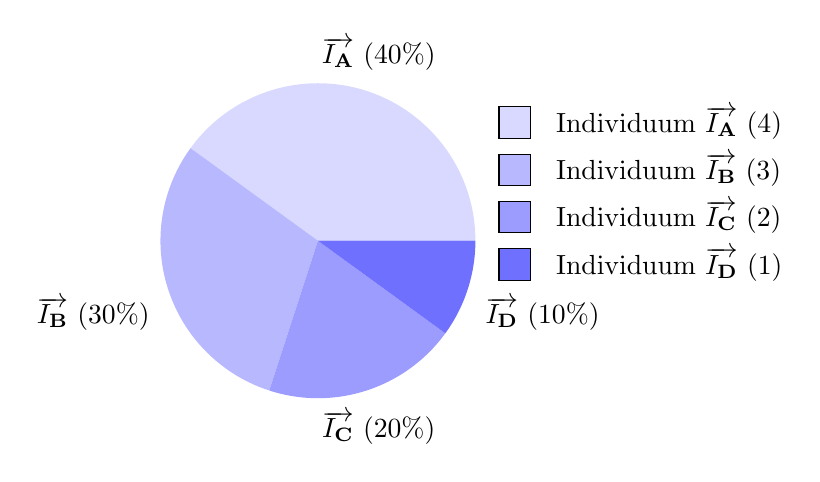
\begin{tikzpicture}
        \def\r{2.0} % radius

        % Example fitness values: A=2, B=3, C=1, D=4 (sum = 10)
        \fill[colorA!75]  (0,0) -- (0:\r)   arc (0:144:\r)   -- cycle; % A (40%)
        \fill[colorB!70]  (0,0) -- (144:\r) arc (144:252:\r) -- cycle; % B (30%)
        \fill[colorC!65]  (0,0) -- (252:\r) arc (252:324:\r) -- cycle; % C (20%)
        \fill[colorD!70]  (0,0) -- (324:\r) arc (324:360:\r) -- cycle; % D (10%)

        \node[anchor=center] at (72:1.25*\r)  {$\overrightarrow{I_{\mathbf{A}}}$ (40\%)};
        \node[anchor=center] at (198:1.5*\r)  {$\overrightarrow{I_{\mathbf{B}}}$ (30\%)};
        \node[anchor=center] at (288:1.25*\r) {$\overrightarrow{I_{\mathbf{C}}}$ (20\%)};
        \node[anchor=center] at (342:1.5*\r)  {$\overrightarrow{I_{\mathbf{D}}}$ (10\%)};

        %\node[font=\bfseries] at (0,-2.8) {Selektion (fitness-proportional)};

        \begin{scope}[shift={(2.3,1.3)}]
        \draw[fill=colorA!75]  (0,0)    rectangle ++(0.4,0.4) node[shift={(0.2,-0.2)},anchor=west] {Individuum $\overrightarrow{I_{\mathbf{A}}}$ (4)};
        \draw[fill=colorB!70]  (0,-0.6) rectangle ++(0.4,0.4) node[shift={(0.2,-0.2)},anchor=west] {Individuum $\overrightarrow{I_{\mathbf{B}}}$ (3)};
        \draw[fill=colorC!65]  (0,-1.2) rectangle ++(0.4,0.4) node[shift={(0.2,-0.2)},anchor=west] {Individuum $\overrightarrow{I_{\mathbf{C}}}$ (2)};
        \draw[fill=colorD!70]  (0,-1.8) rectangle ++(0.4,0.4) node[shift={(0.2,-0.2)},anchor=west] {Individuum $\overrightarrow{I_{\mathbf{D}}}$ (1)};
        \end{scope}
    \end{tikzpicture}
    \caption{Selektion von Individuen basierend auf ihrer Fitness}
    \label{fig:GeneticAlgo_Selection}
    \end{figure}
}


\minipagedOrBelowEachOther
{
    \vspace{1cm}
    Zwei selektierte Eltern werden in~\ref{fig:GeneticAlgo_SelectionPair} dargestellt.
    Dabei repräsentieren die Kästchen die Gene der Individuen, 
    welche die zu optimierenden Parameter $k_{\mathbf{ij}}$ darstellen.
}{

\begin{figure}[H]
\centering
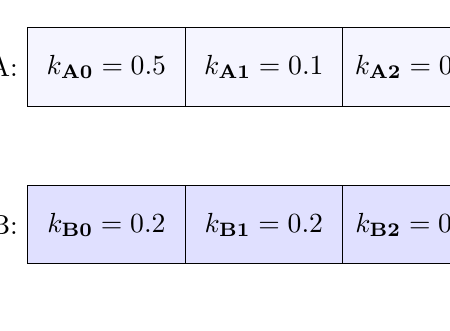
\begin{tikzpicture}
    \useasboundingbox (0,1) rectangle (5,-2.5); % define bounding box to avoid cropping
    \def\vsize{1.0} % vertical size of the box
    \def\hsize{2} % horizontal size of each gene box

    
    

    %\begin{scope}[shift={(3.0,5.0)}]
        \node[anchor=east] at (0, \vsize*0.5) {Elternteil A:};
        \draw[fill=lightGenomColor!20] (0*\hsize,0) rectangle ++(\hsize,\vsize) node[shift={(-\hsize*0.5,-\vsize*0.5)},anchor=center]{$k_{\mathbf{A0}}=0.5$};
        \draw[fill=lightGenomColor!20] (1*\hsize,0) rectangle ++(\hsize,\vsize) node[shift={(-\hsize*0.5,-\vsize*0.5)},anchor=center]{$k_{\mathbf{A1}}=0.1$};
        \draw[fill=lightGenomColor!20] (2*\hsize,0) rectangle ++(\hsize,\vsize) node[shift={(-\hsize*0.5,-\vsize*0.5)},anchor=center]{$k_{\mathbf{A2}}=0.01$};

        \node[anchor=east] at (0, -\vsize*1.5) {Elternteil B:};
        \draw[fill=darkGenomColor!20] (0*\hsize,-\vsize*2) rectangle ++(\hsize,\vsize) node[shift={(-\hsize*0.5,-\vsize*0.5)},anchor=center]{$k_{\mathbf{B0}}=0.2$};
        \draw[fill=darkGenomColor!20] (1*\hsize,-\vsize*2) rectangle ++(\hsize,\vsize) node[shift={(-\hsize*0.5,-\vsize*0.5)},anchor=center]{$k_{\mathbf{B1}}=0.2$};
        \draw[fill=darkGenomColor!20] (2*\hsize,-\vsize*2) rectangle ++(\hsize,\vsize) node[shift={(-\hsize*0.5,-\vsize*0.5)},anchor=center]{$k_{\mathbf{B2}}=0.05$};
        %\node[font=\bfseries, anchor=center] at (\hsize*1.5,-\vsize*2-0.5) {Selektiertes Paar};
    %\end{scope}
\end{tikzpicture}   
\caption{Selektierte Eltern für die Kreuzung}
\label{fig:GeneticAlgo_SelectionPair}
\end{figure}
}
\horizontalLine


\minipagedWithHFillOrBelowEachOther
{
        \subparagraph{Kreuzung}
        \noindent
        \\
        \begin{figure}[H]
        \centering
        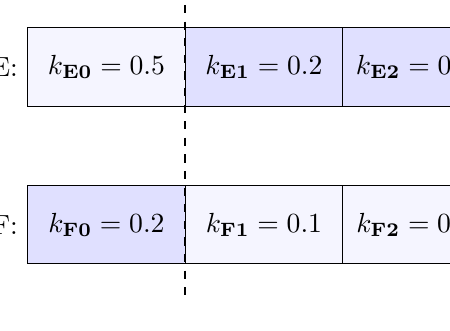
\begin{tikzpicture}
            \useasboundingbox (0,1) rectangle (5,-2.5); % define bounding box to avoid cropping
            \def\vsize{1.0} % vertical size of the box
            \def\hsize{2} % horizontal size of each gene box

            %\begin{scope}[shift={(3.0,-5.0)}]
                \node[anchor=east] at (0, \vsize*0.5) {Kind E:};
                \draw[fill=lightGenomColor!20] (0*\hsize,0) rectangle ++(\hsize,\vsize) node[shift={(-\hsize*0.5,-\vsize*0.5)},anchor=center]{$k_{\mathbf{E0}}=0.5$};
                \draw[fill=darkGenomColor!20] (1*\hsize,0) rectangle ++(\hsize,\vsize) node[shift={(-\hsize*0.5,-\vsize*0.5)},anchor=center]{$k_{\mathbf{E1}}=0.2$};
                \draw[fill=darkGenomColor!20] (2*\hsize,0) rectangle ++(\hsize,\vsize) node[shift={(-\hsize*0.5,-\vsize*0.5)},anchor=center]{$k_{\mathbf{E2}}=0.05$};

                \node[anchor=east] at (0, -\vsize*1.5) {Kind F:};
                \draw[fill=darkGenomColor!20] (0*\hsize,-\vsize*2) rectangle ++(\hsize,\vsize) node[shift={(-\hsize*0.5,-\vsize*0.5)},anchor=center]{$k_{\mathbf{F0}}=0.2$};
                \draw[fill=lightGenomColor!20] (1*\hsize,-\vsize*2) rectangle ++(\hsize,\vsize) node[shift={(-\hsize*0.5,-\vsize*0.5)},anchor=center]{$k_{\mathbf{F1}}=0.1$};
                \draw[fill=lightGenomColor!20] (2*\hsize,-\vsize*2) rectangle ++(\hsize,\vsize) node[shift={(-\hsize*0.5,-\vsize*0.5)},anchor=center]{$k_{\mathbf{F2}}=0.01$};
            % \node[font=\bfseries, anchor=center] at (\hsize*1.5,-\vsize*2-0.5) {Kreuzung (Crossover)};

                % Crossover point as vertical line
                \draw[dashed, thick] (1*\hsize, 1.5) -- (1*\hsize, -\vsize*2-0.5);
            %\end{scope}
        \end{tikzpicture}   
        \caption{Kreuzung (Crossover) zweier Eltern zur Erzeugung von Nachkommen}
        \label{fig:GeneticAlgo_Crossover}
        \end{figure}

        Bei der Kreuzung wird das Genom der beiden Eltern an einer zufälligen Stelle geteilt.
        In \ref{fig:GeneticAlgo_Crossover} ist dies durch die gestrichelte Linie dargestellt.
        Die beiden Teile der Gene werden dann vertauscht, um zwei neue Nachkommen zu erzeugen.
        Dies ermöglicht die Kombination von genetischem Material beider Eltern.
}
{
    \subparagraph{Mutation}
    \noindent
    \\

    \begin{figure}[H]
    \centering
    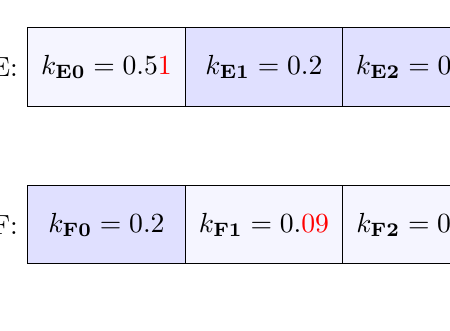
\begin{tikzpicture}
        \useasboundingbox (0,1) rectangle (5,-2.5); % define bounding box to avoid cropping
        \def\vsize{1.0} % vertical size of the box
        \def\hsize{2} % horizontal size of each gene box

        %\begin{scope}[shift={(3.0,-5.0)}]
            \node[anchor=east] at (0, \vsize*0.5) {Kind E:};
            \draw[fill=lightGenomColor!20] (0*\hsize,0) rectangle ++(\hsize,\vsize) node[shift={(-\hsize*0.5,-\vsize*0.5)},anchor=center]{$k_{\mathbf{E0}}=0.5\textcolor{red}{1}$};
            \draw[fill=darkGenomColor!20] (1*\hsize,0) rectangle ++(\hsize,\vsize) node[shift={(-\hsize*0.5,-\vsize*0.5)},anchor=center]{$k_{\mathbf{E1}}=0.2$};
            \draw[fill=darkGenomColor!20] (2*\hsize,0) rectangle ++(\hsize,\vsize) node[shift={(-\hsize*0.5,-\vsize*0.5)},anchor=center]{$k_{\mathbf{E2}}=0.05$};

            \node[anchor=east] at (0, -\vsize*1.5) {Kind F:};
            \draw[fill=darkGenomColor!20] (0*\hsize,-\vsize*2) rectangle ++(\hsize,\vsize) node[shift={(-\hsize*0.5,-\vsize*0.5)},anchor=center]{$k_{\mathbf{F0}}=0.2$};
            \draw[fill=lightGenomColor!20] (1*\hsize,-\vsize*2) rectangle ++(\hsize,\vsize) node[shift={(-\hsize*0.5,-\vsize*0.5)},anchor=center]{$k_{\mathbf{F1}}=0.\textcolor{red}{09}$};
            \draw[fill=lightGenomColor!20] (2*\hsize,-\vsize*2) rectangle ++(\hsize,\vsize) node[shift={(-\hsize*0.5,-\vsize*0.5)},anchor=center]{$k_{\mathbf{F2}}=0.01$};
        % \node[font=\bfseries, anchor=center] at (\hsize*1.5,-\vsize*2-0.5) {Kreuzung (Crossover)};

        %\end{scope}
    \end{tikzpicture}   
    \caption{Mutation von Genen in den Nachkommen}
    \label{fig:GeneticAlgo_Mutation}
    \end{figure}
    Bei der Mutation werden an den Nachkommen zufällige Änderungen an einzelnen Genen vorgenommen.
    In \ref{fig:GeneticAlgo_Mutation} sind die mutierten Gene rot hervorgehoben.
    Wie viele Gene mutieren und wie stark sie verändert werden, hängt von der Mutationschance und der Mutationsrate ab.

    % mathematisch ausgedrückt:
    \begin{equation}
    k_{\mathbf{ij\_neu}} =
    \begin{cases}
    k_{\mathbf{ij}} + \alpha \cdot \mathFunction{randN}{-1, 1} & \text{wenn } \mathFunction{randG}{0,1} < \beta \\
    k_{\mathbf{ij}} & \text{sonnst}
    \end{cases}
    \end{equation}
    \[
        \mathFunction{randG}{a,b} \text{ ist eine gleichverteilte Zufallsvariable im Intervall [a, b] } 
    \]
    \[
        \mathFunction{randN}{a, b} \text{ ist eine normalverteilte Zufallsvariable im Intervall [a, b] } 
    \]
}

\horizontalLine

\minipagedWithHFillOrBelowEachOther
{
   
        \subparagraph{Ersetzung}
        \noindent
        \\
        Nach der Bewertung der neuen Generation von Individuen,
        werden die Individuen der alten Generation durch die neuen Individuen ersetzt.
        Dies geschieht in der Regel vollständig, wobei die gesamte alte Population durch die neue Population ersetzt wird.
}
{
         \subparagraph{Abbruchbedingung}
        \noindent
        \\
        Der Optimierungsprozess wird wiederholt, bis eine Abbruchbedingung erfüllt ist.
        Dies kann eine vordefinierte Anzahl von Generationen sein,
        eine bestimmte Fitness-Schwelle, die erreicht werden muss,
        oder eine Kombination aus beiden.
        Sobald die Abbruchbedingung erfüllt ist,
        wird das beste Individuum in der Population als die optimale Lösung des Problems betrachtet.
}

\newpage


\paragraph{Einfluss der Startbedingungen und Hyperparameter}
Massgeblich für den Erfolg eines guten Resultates sind folgende Parameter beteiligt:
\begin{itemize}
    \item Populationsgrösse, also die Anzahl der Individuen
    \item Streuung der Gene in der Startpopulation, also wie unterschiedlich die Individuen zu Beginn sind
    \item Mutationschance, also wie häufig Gene zufällig verändert werden
    \item Mutationsrate, also wie stark die Gene bei einer Mutation verändert werden
    \item Anzahl Generationen
\end{itemize}

\horizontalLine
\subparagraph{Populationsgrösse}
\noindent
\\
\minipagedOrBelowEachOther
{
Wie in der Natur auch, ist eine grössere Population vorteilhaft um eine grössere genetische Vielfalt 
zu gewährleisten. Dies erhöht die Wahrscheinlichkeit, dass gute Lösungen gefunden werden.
}{
Allerdings steigt mit der Populationsgrösse auch der Rechenaufwand pro Generation, 
da mehr Individuen bewertet werden müssen.
}

\horizontalLine

\subparagraph{Streuung der Startpopulation}
\noindent
\\
\begin{figure}[H]
    \centering
    \begin{minipage}{0.48\textwidth}
        \centering
        %\centering
        \includegraphics[width=\linewidth]{images/Genetic2DProblemSpaceVisualisation_1.pdf}
        \caption{Geringe Streuung der Startpopulation in einem 2D Problemraum}
        \label{fig:Genetic2DProblemSpaceVisualisation_1}
    \end{minipage}\hfill
    \begin{minipage}{0.48\textwidth}
        \centering
       % \centering
        \vspace{-0.2cm}
        \includegraphics[width=\linewidth]{images/Genetic2DProblemSpaceVisualisation_2.pdf}
        \caption{Hohe Streuung der Startpopulation in einem 2D Problemraum}
        \label{fig:Genetic2DProblemSpaceVisualisation_2}
    \end{minipage}
\end{figure}

\minipagedOrBelowEachOther
{
    Die Streuung der Startpopulation beeinflusst die genetische Vielfalt der Individuen zu Beginn des Optimierungsprozesses.
    Eine kleine Streuung, wie in~\ref{fig:Genetic2DProblemSpaceVisualisation_1} dargestellt,
    kann dazu führen, dass der Algorithmus in lokalen Optima stecken bleibt,
    da die Individuen zu ähnlich sind und somit nicht genügend Vielfalt vorhanden ist, um den Suchraum effektiv zu erkunden.
}{
    Eine hohe Streuung, wie in~\ref{fig:Genetic2DProblemSpaceVisualisation_2} dargestellt,
    ermöglicht es dem Algorithmus, verschiedene Bereiche des Suchraums zu erkunden.
    Dies erhöht die Chancen, globale Optima zu finden, da die Individuen unterschiedliche Lösungen repräsentieren.

    Über den Verlauf der Optimierung hinweg, tendiert die Streuung der Population dazu abzunehmen.
    Wie gross die Streuung der Population langfristig ist, hängt von der Mutationschance und der Mutationsrate ab.
}
\horizontalLine

\minipagedWithHFillOrBelowEachOther
{

        \subparagraph{Mutationschance \(\beta\)}
        \noindent
        \\
        Die Mutationschance bestimmt, wie häufig Gene zufällig verändert werden.
        Während des Mutationsschrittes wird für jedes Gen, also für jeden Optimierungsparameter eines Individuums, 
        entschieden, ob es mutiert oder nicht. Eine höhere Mutationschance führt zu einer grösseren genetischen Vielfalt in der Population.
        Es ist jedoch nicht ratsam die Mutationschance zu hoch zu wählen, da dies den Suchprozess zu zufällig machen kann.
        Zu viele Mutationen auf einmal sind kontraproduktiv da jeder Parameter Einfluss auf eine gute Lösung hat und
        zu viele Veränderungen auf einmal, die Chance erhöht eine bereits gute Lösung zu verschlechtern.
}
{
        \subparagraph{Mutationsrate \(\alpha\)}
        \noindent
        \\
        Die Mutationsrate bestimmt, wie stark die Gene bei einer Mutation verändert werden.
        Ein Gen wird bei der Mutation immer um einen zufälligen Wert verändert, der durch die Mutationsrate skaliert wird.
        Eine höhere Mutationsrate führt zu grösseren Veränderungen der Gene, was die genetische Vielfalt erhöht.
        Allerdings kann eine zu hohe Mutationsrate dazu führen, dass gute Lösungen zerstört werden,
        da die Veränderungen zu drastisch sind.
        Die Mutationsrate wird optimalerweise im Verlauf der Optimierung verringert,
        um zu Beginn eine breite Suche zu ermöglichen und später die Suche zu verfeinern.
}


%\begin{figure}[H]
%    \centering
%    \includegraphics[width=\linewidth*2/3]{images/Genetic2DProblemSpaceVisualisation_1.pdf}
%    \caption{Geringe Streuung der Startpopulation in einem 2D Problemraum}
%    \label{fig:Genetic2DProblemSpaceVisualisation_1}
%\end{figure}
%
%\begin{figure}[H]
%    \centering
%    \includegraphics[width=\linewidth*2/3]{images/Genetic2DProblemSpaceVisualisation_2.pdf}
%    \caption{Hohe Streuung der Startpopulation in einem 2D Problemraum}
%    \label{fig:Genetic2DProblemSpaceVisualisation_2}
%\end{figure}


\newpage
\subparagraph{Warum die Fitnessfunktion einen positiven Wert generieren muss}
\noindent
\\
\label{sec:Description_GenetischerAlgorithmus_FitnessFunction}
\minipagedOrBelowEachOther
{
    Bei der Selektion der Individuen für die Paarung wird die Fitness jedes Individuums verwendet.
    Die Wahrscheinlichkeit, dass ein Individuum ausgewählt wird, ist proportional zu seiner Fitness und ist definiert als:
    \begin{equation}
    \mathFunction{P}{\overrightarrow{I_{\mathbf{i}}}} = \frac{\mathFunction{f}{\overrightarrow{I_{\mathbf{i}}}}}{\sum_{j=0}^{N-1} \mathFunction{f}{\overrightarrow{I_{\mathbf{j}}}}}
    \end{equation}
    Wobei $\mathFunction{P}{\overrightarrow{I_{\mathbf{i}}}}$ die Selektionswahrscheinlichkeit des Individuums $\overrightarrow{I_{\mathbf{i}}}$ ist,
    $\mathFunction{f}{\overrightarrow{I_{\mathbf{i}}}}$ die Fitness des Individuums $\overrightarrow{I_{\mathbf{i}}}$ ist und
    $N$ die Gesamtanzahl der Individuen in der Population ist.
}{
    Mit negativen Fitnesswerten lassen sich keine Wahrscheinlichkeiten berechnen,
    da nach dieser Formel die Wahrscheinlichkeit, 
    selektiert zu werden auch negativ werden könnte, was keinen Sinn ergibt.
    Daher muss die Fitnessfunktion so definiert werden, dass sie immer einen positiven Wert zurückgibt.

    Es ist ausserdem auch schwierig ein \gls{Minimierungsproblem} mit diesem Selektierungsverfahren zu lösen,
    da eine geringere Fitness zu einer höheren Selektionswahrscheinlichkeit führen müsste.

    Es gibt Methoden wie man ein Minimierungsproblem zu einem \gls{Maximierungsproblem} umwandeln kann.
}

\horizontalLine
\minipagedOrBelowEachOther
{
    \subparagraph{Vorzeichen wechseln}
    \noindent
    \\
    Durch das wechseln des Vorzeichens der Bewertungsfunktion, \\
    also $\mathFunction{f}{\overrightarrow{x}} = -\mathFunction{g}{\overrightarrow{x}}$,
    wird aus einem Minimierungsproblem ein \\
    Maximierungsproblem.
}{
    \subparagraph{Problematik}
    \noindent
    \\
    Dabei können jedoch negative Fitnesswerte entstehen, \\
    wenn die Bewertungsfunktion $\mathFunction{g}{\overrightarrow{x}}$ positive Werte annimmt.
}

\horizontalLine
\subparagraph{Vorzeichen wechseln und verschieben}
\noindent
\\

\newcommand{\geneticPlotScale}{0.8}
\newcommand{\geneticPlotLabelYoffset}{0.4}
\newcommand{\geneticFitnessA}{10}
\newcommand{\geneticFitnessB}{5}
\newcommand{\geneticFitnessC}{2}
\newcommand{\geneticFitnessD}{1}

\newcommand{\geneticFitnessOffset}{11}
\newcommand{\geneticFitnessScale}{0.4}

\begin{figure}[H]
    \centering
    \begin{minipage}{0.45\textwidth}
        \centering
        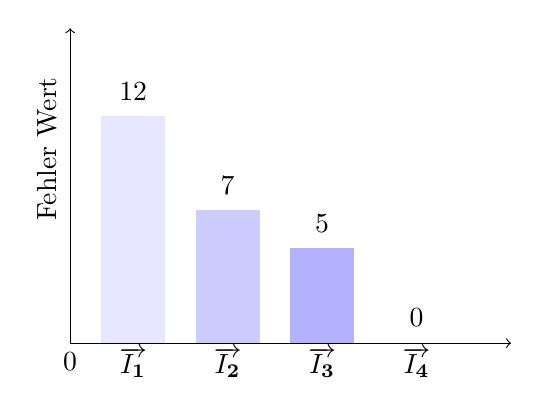
\begin{tikzpicture}[scale=\geneticPlotScale]
            % x-axis label at 0
            \node[below] at (0,0) {0};

            % Bars with numeric labels
            % Bar A
            \filldraw[colorA!50] (0.5,0) rectangle (1.5,\geneticFitnessA*\geneticFitnessScale);
            \node at (1.0,\geneticFitnessA*\geneticFitnessScale+\geneticPlotLabelYoffset) {\geneticFitnessA};

            % Bar B
            \filldraw[colorB!50] (2.0,0) rectangle (3.0,\geneticFitnessB*\geneticFitnessScale);
            \node at (2.5,\geneticFitnessB*\geneticFitnessScale+\geneticPlotLabelYoffset) {\geneticFitnessB};
            % Bar C
            \filldraw[colorC!50] (3.5,0) rectangle (4.5,\geneticFitnessC*\geneticFitnessScale);
            \node at (4.0,\geneticFitnessC*\geneticFitnessScale+\geneticPlotLabelYoffset) {\geneticFitnessC};

            % Bar D
            \filldraw[colorD!50] (5.0,0) rectangle (6.0,\geneticFitnessD*\geneticFitnessScale);
            \node at (5.5,\geneticFitnessD*\geneticFitnessScale+\geneticPlotLabelYoffset) {\geneticFitnessD};
            % Category labels
            \node at (1.0,-0.3) {$\overrightarrow{I_{\mathbf{1}}}$};
            \node at (2.5,-0.3) {$\overrightarrow{I_{\mathbf{2}}}$};
            \node at (4.0,-0.3) {$\overrightarrow{I_{\mathbf{3}}}$};
            \node at (5.5,-0.3) {$\overrightarrow{I_{\mathbf{4}}}$};

            % Axes
            \draw[->] (0,0) -- (7,0);% node[below]{Individuen};
            \draw[->] (0,0) -- (0,5) node[left, rotate=90, shift={(-0.5,0.3)}]{Fehler Wert};
        \end{tikzpicture}
        \caption{Originale Fehlerwerte der Individuen}
        %\label{fig:GeneticAlgo_FitnessValues_Original}

        % Math formula table
        %\begin{tabular}{c}
        %    $\mathbf{P}(I_{\mathbf{A}}) = \frac{f(I_{\mathbf{A}})}{\sum_{j=0}^{N-1} f(I_{\mathbf{j}})} = \frac{10}{10 + 5 + 2 + 1} = 0.55$ \\
        %    $\mathbf{P}(I_{\mathbf{B}}) = \frac{f(I_{\mathbf{B}})}{\sum_{j=0}^{N-1} f(I_{\mathbf{j}})} = \frac{5}{10 + 5 + 2 + 1} = 0.27$ \\
        %    $\mathbf{P}(I_{\mathbf{C}}) = \frac{f(I_{\mathbf{C}})}{\sum_{j=0}^{N-1} f(I_{\mathbf{j}})} = \frac{2}{10 + 5 + 2 + 1} = 0.11$ \\
        %    $\mathbf{P}(I_{\mathbf{D}}) = \frac{f(I_{\mathbf{D}})}{\sum_{j=0}^{N-1} f(I_{\mathbf{j}})} = \frac{1}{10 + 5 + 2 + 1} = 0.05$ \\
        %\end{tabular}  
    \end{minipage}
    \hfill $\longrightarrow$ \hfill
    \begin{minipage}{0.45\textwidth}
        \centering
        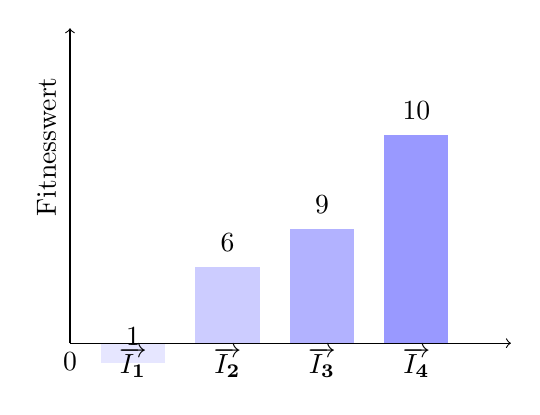
\begin{tikzpicture}[scale=\geneticPlotScale]
            % x-axis label at 0
            \node[below] at (0,0) {0};

            % Bars with numeric labels
            % Bar A
            \filldraw[colorA!50] (0.5,0) rectangle (1.5,\geneticFitnessOffset*\geneticFitnessScale-\geneticFitnessA*\geneticFitnessScale);
            \node at (1.0,-\geneticFitnessA*\geneticFitnessScale + \geneticFitnessOffset*\geneticFitnessScale +\geneticPlotLabelYoffset) {1};

            % Bar B
            \filldraw[colorB!50] (2.0,0) rectangle (3.0,-\geneticFitnessB*\geneticFitnessScale + \geneticFitnessOffset*\geneticFitnessScale);
            \node at (2.5,-\geneticFitnessB*\geneticFitnessScale + \geneticFitnessOffset*\geneticFitnessScale +\geneticPlotLabelYoffset) {6};
            % Bar C
            \filldraw[colorC!50] (3.5,0) rectangle (4.5,-\geneticFitnessC*\geneticFitnessScale + \geneticFitnessOffset*\geneticFitnessScale);
            \node at (4.0,-\geneticFitnessC*\geneticFitnessScale + \geneticFitnessOffset*\geneticFitnessScale +\geneticPlotLabelYoffset) {9};
            % Bar D
            \filldraw[colorD!50] (5.0,0) rectangle (6.0,-\geneticFitnessD*\geneticFitnessScale + \geneticFitnessOffset*\geneticFitnessScale);
            \node at (5.5,-\geneticFitnessD*\geneticFitnessScale + \geneticFitnessOffset*\geneticFitnessScale +\geneticPlotLabelYoffset) {10};
            % Category labels
            \node at (1.0,-0.3) {$\overrightarrow{I_{\mathbf{1}}}$};
            \node at (2.5,-0.3) {$\overrightarrow{I_{\mathbf{2}}}$};
            \node at (4.0,-0.3) {$\overrightarrow{I_{\mathbf{3}}}$};
            \node at (5.5,-0.3) {$\overrightarrow{I_{\mathbf{4}}}$};

            % Axes
            \draw[->] (0,0) -- (7,0);% node[below]{Individuen};
            \draw[->] (0,0) -- (0,5) node[left, rotate=90, shift={(-0.5,0.3)}]{Fitnesswert};
        \end{tikzpicture}
        \caption{Vorzeichenwechsel + Verschiebung}
        %\label{fig:GeneticAlgo_FitnessValues_Transformed}
        % Math formula table
        %\begin{tabular}{c}
        %    $\mathbf{P}(I_{\mathbf{A}}) = \frac{C - f(I_{\mathbf{A}})}{\sum_{j=0}^{N-1} (C - f(I_{\mathbf{j}}))} = \frac{1}{1 + 6 + 9 + 10} = 0.03$ \\
        %    $\mathbf{P}(I_{\mathbf{B}}) = \frac{C - f(I_{\mathbf{B}})}{\sum_{j=0}^{N-1} (C - f(I_{\mathbf{j}}))} = \frac{6}{1 + 6 + 9 + 10} = 0.23$ \\
        %    $\mathbf{P}(I_{\mathbf{C}}) = \frac{C - f(I_{\mathbf{C}})}{\sum_{j=0}^{N-1} (C - f(I_{\mathbf{j}}))} = \frac{9}{1 + 6 + 9 + 10} = 0.34$ \\
        %    $\mathbf{P}(I_{\mathbf{D}}) = \frac{C - f(I_{\mathbf{D}})}{\sum_{j=0}^{N-1} (C - f(I_{\mathbf{j}}))} = \frac{10}{1 + 6 + 9 + 10} = 0.38$ \\
        %\end{tabular}
    \end{minipage}
\end{figure}

\minipagedOrBelowEachOther
{
    Um sicherzustellen, dass die Fitnessfunktion immer positive Werte zurückgibt,
    kann die Bewertungsfunktion um einen konstanten Wert verschoben werden.
    \begin{equation}
    \mathFunction{f}{\overrightarrow{x}} = -\mathFunction{g}{\overrightarrow{x}} + C
    \end{equation}
    
}{
    Offset $C$ ist beispielsweise als 11 gewählt worden, \\
    da ansonsten Individuum A auf 0 kommen würde. 
    $\rightarrow$ Somit hätte Individuum A keine Chance selektiert zu werden, was nicht fair ist.
}

\subparagraph{Problematik}
\noindent
\\

%\[
%    \lim_{C \to \infty} \mathbf{P}(I_{\mathbf{i}}) 
%    = \lim_{C \to \infty} \frac{C - f(I_{\mathbf{i}})}{\sum_{j=0}^{N-1} (C - f(I_{\mathbf{j}}))} 
%    = \lim_{C \to \infty} \frac{C}{\sum_{j=0}^{N-1} C} 
%    = \lim_{C \to \infty} \frac{C}{N \cdot C} 
%    = \frac{1}{N} \quad \forall i \in [0, N-1]
%\]

\minipagedOrBelowEachOther
{
	%\vspace{0.4cm}
	Mit dem benötigten Offset $C$ werden die Verhältnisse der Fitnesswerte zueinander verändert.
    Wird ein zu grosses $C$ gewählt, so werden die Unterschiede zwischen den Fitnesswerten immer kleiner.
    Dadurch erhalten alle Individuen eine ähnliche Selektionswahrscheinlichkeit, 
    was sich negativ auf die Effizienz des \gls{GA} auswirkt.
}{
	%\centering
    \begin{equation}
    \lim_{C \to \infty} \mathbf{P}(\overrightarrow{I_{\mathbf{i}}}) 
        = \lim_{C \to \infty} \frac{C - f(\overrightarrow{I_{\mathbf{i}}})}{\sum_{j=0}^{N-1} \left(C - f(\overrightarrow{I_{\mathbf{j}}})\right)} 
        \quad \forall i \in [0, N-1]
    \end{equation}
    \begin{equation}
        = \lim_{C \to \infty} \frac{C}{\sum_{j=0}^{N-1} C} 
    \end{equation}
    \begin{equation}
        = \lim_{C \to \infty} \frac{C}{N \cdot C} = \frac{1}{N} 
    \end{equation}
}


\newpage %\horizontalLine
\subparagraph{Verschiebung und Invertierung der Fitnesswerte}
\label{sec:Description_GenetischerAlgorithmus_FitnessFunction_Transformation_Invert}
\noindent
\\
\infoBlock{Die folgende Methode ist in der C++ Implementierung umgesetzt und wird angewendet, 
wenn die Bewertungsfunktion als Minimierungsproblem definiert ist.}


Eine weitere Möglichkeit besteht darin, alle Fitnesswerte um den niedrigsten Fitnesswert in den positiven Bereich 
zu verschieben und anschliessend zu invertieren.
% Notiz



\begin{figure}[H]
    \centering
    \begin{tabular}{@{}clr@{}}
            \toprule
            \textbf{Symbol} & \textbf{Beschreibung} \\
            \midrule
            $g(\overrightarrow{I_{\mathbf{i}}})$ & Fehler-Minimierungs-Funktion.  $g(\overrightarrow{I_{\mathbf{i}}}) \in \mathbb{R}$ \\[0.5ex]
            $\delta$            & Konstanter Wert zur Verschiebung der Fitnesswerte. $\delta = \varepsilon, \varepsilon > 0 \land \varepsilon \to 0$\\
            \bottomrule
    \end{tabular}
    \caption{Symbole für die Fitnessfunktion Transformation}
\end{figure}

Bei der Anwendung des \gls{GA} muss die Fehler-Minimierungs-Funktion $g(\overrightarrow{I_{\mathbf{i}}})$ gegeben sein.
Damit diese vom \gls{GA} verwendet werden kann, muss sie in eine Maximierungs-Fitness-Funktion $f(\overrightarrow{I_{\mathbf{i}}})$ umgewandelt werden.
Bei der Umwandlung müssen jedoch einige Kompromisse in Kauf genommen werden:
\begin{itemize}
    \item Die Verhältnisse der Fitnesswerte zueinander werden verändert.
    \item Das schlechteste Individuum erhält eine Fitness von 0 und hat somit keine Chance selektiert zu werden.
    \item Bei sehr ähnlichen Fehlerwerten steigt der Einfluss von $\delta$ auf die Wahrscheinlichkeiten der einzelnen Individuen.
\end{itemize}


\horizontalLine
\subparagraph{Vorgehen bei der Umwandlung $g(\overrightarrow{I_{\mathbf{i}}}) \rightarrow f(\overrightarrow{I_{\mathbf{i}}})$}
\noindent
\\
%\horizontalLine
\label{sec:Description_GenetischerAlgorithmus_FitnessFunction_TransformationSteps}


\renewcommand{\geneticFitnessA}{-2}
\renewcommand{\geneticFitnessB}{3}
\renewcommand{\geneticFitnessC}{5}
\renewcommand{\geneticFitnessD}{10}
\renewcommand{\geneticFitnessScale}{0.3}
\begin{figure}[H]
    %\centering
    \begin{minipage}{0.48\textwidth}
        \vspace{-1cm}
        Als erstes wird der niedrigste Fehlerwert bestimmt:
        \begin{equation}
            g_{\mathbf{min}} = \min_{i \in [0, N-1]}(g(\overrightarrow{I_{\mathbf{i}}})) = -2
        \end{equation}
        Wenn dieser negativ ist, werden alle Fehlerwerte um den Betrag des niedrigsten Wertes verschoben:
        \begin{equation}
            g_{\mathbf{shift}}(\overrightarrow{I_{\mathbf{i}}}) =
            \begin{cases}
                g(\overrightarrow{I_{\mathbf{i}}}) - g_{\mathbf{min}} & \text{if}(g_{\mathbf{min}} < 0) \\
                g(\overrightarrow{I_{\mathbf{i}}}) & \text{sonnst}
            \end{cases}
        \end{equation}
       
    \end{minipage}\hfill
    \begin{minipage}{0.48\textwidth}
        \centering
        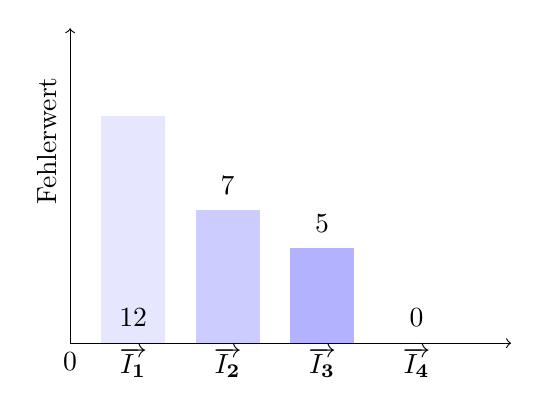
\begin{tikzpicture}[scale=\geneticPlotScale]
            % x-axis label at 0
            \node[below] at (0,0) {0};

            % Bars with numeric labels
            % Bar A
            \filldraw[colorA!50] (0.5,0) rectangle (1.5,\geneticFitnessA*\geneticFitnessScale);
            \node at (1.0,\geneticPlotLabelYoffset) {\geneticFitnessA};

            % Bar B
            \filldraw[colorB!50] (2.0,0) rectangle (3.0,\geneticFitnessB*\geneticFitnessScale);
            \node at (2.5,\geneticFitnessB*\geneticFitnessScale+\geneticPlotLabelYoffset) {\geneticFitnessB};
            % Bar C
            \filldraw[colorC!50] (3.5,0) rectangle (4.5,\geneticFitnessC*\geneticFitnessScale);
            \node at (4.0,\geneticFitnessC*\geneticFitnessScale+\geneticPlotLabelYoffset) {\geneticFitnessC};

            % Bar D
            \filldraw[colorD!50] (5.0,0) rectangle (6.0,\geneticFitnessD*\geneticFitnessScale);
            \node at (5.5,\geneticFitnessD*\geneticFitnessScale+\geneticPlotLabelYoffset) {\geneticFitnessD};
            % Category labels
            \node at (1.0,-0.3) {$\overrightarrow{I_{\mathbf{1}}}$};
            \node at (2.5,-0.3) {$\overrightarrow{I_{\mathbf{2}}}$};
            \node at (4.0,-0.3) {$\overrightarrow{I_{\mathbf{3}}}$};
            \node at (5.5,-0.3) {$\overrightarrow{I_{\mathbf{4}}}$};

            % Axes
            \draw[->] (0,0) -- (7,0); % node[below]{Individuen};
            \draw[->] (0,0) -- (0,5) node[left, rotate=90, shift={(-0.5,0.3)}]{Fehlerwert};
        \end{tikzpicture}
        \caption{Fehlerwerte der Individuen $g(\overrightarrow{I_{\mathbf{i}}})$}
    \end{minipage}
\end{figure}


\horizontalLine

\renewcommand{\geneticFitnessA}{0}
\renewcommand{\geneticFitnessB}{5}
\renewcommand{\geneticFitnessC}{7}
\renewcommand{\geneticFitnessD}{12}
\begin{figure}[H]
    %\centering
    \begin{minipage}{0.48\textwidth}
        \vspace{-1cm}
        Für den nächsten Schritt wird der maximale Fehlerwert benötigt:
        \begin{equation}
            g_{\mathbf{shift\_max}} = \max_{i \in [0, N-1]}(g_{\mathbf{shift}}(\overrightarrow{I_{\mathbf{i}}})) = 12
        \end{equation}
        Nun werden die Fehlerwerte am maximalen Fehlerwert invertiert, 
        um eine Maximierungs-Fitness-Funktion zu erhalten.
        \begin{equation}
            g_{\mathbf{invert}}(\overrightarrow{I_{\mathbf{i}}}) = g_{\mathbf{shift\_max}} - g_{\mathbf{shift}}(\overrightarrow{I_{\mathbf{i}}})
        \end{equation}
       
    \end{minipage}\hfill
    \begin{minipage}{0.48\textwidth}
        \centering
        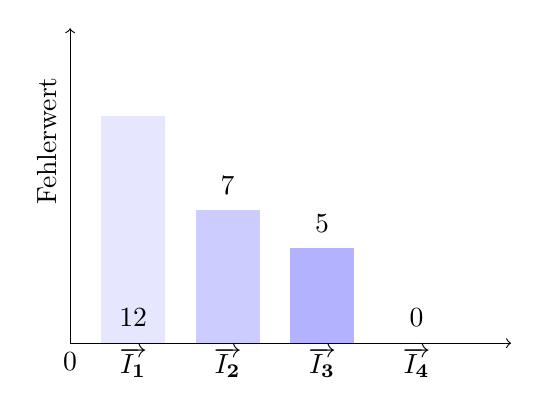
\begin{tikzpicture}[scale=\geneticPlotScale]
            % x-axis label at 0
            \node[below] at (0,0) {0};

            % Bars with numeric labels
            % Bar A
            \filldraw[colorA!50] (0.5,0) rectangle (1.5,\geneticFitnessA*\geneticFitnessScale);
            \node at (1.0,\geneticPlotLabelYoffset) {\geneticFitnessA};

            % Bar B
            \filldraw[colorB!50] (2.0,0) rectangle (3.0,\geneticFitnessB*\geneticFitnessScale);
            \node at (2.5,\geneticFitnessB*\geneticFitnessScale+\geneticPlotLabelYoffset) {\geneticFitnessB};
            % Bar C
            \filldraw[colorC!50] (3.5,0) rectangle (4.5,\geneticFitnessC*\geneticFitnessScale);
            \node at (4.0,\geneticFitnessC*\geneticFitnessScale+\geneticPlotLabelYoffset) {\geneticFitnessC};

            % Bar D
            \filldraw[colorD!50] (5.0,0) rectangle (6.0,\geneticFitnessD*\geneticFitnessScale);
            \node at (5.5,\geneticFitnessD*\geneticFitnessScale+\geneticPlotLabelYoffset) {\geneticFitnessD};
            % Category labels
            \node at (1.0,-0.3) {$\overrightarrow{I_{\mathbf{1}}}$};
            \node at (2.5,-0.3) {$\overrightarrow{I_{\mathbf{2}}}$};
            \node at (4.0,-0.3) {$\overrightarrow{I_{\mathbf{3}}}$};
            \node at (5.5,-0.3) {$\overrightarrow{I_{\mathbf{4}}}$};

            % Axes
            \draw[->] (0,0) -- (7,0); % node[below]{Individuen};
            \draw[->] (0,0) -- (0,5) node[left, rotate=90, shift={(-0.5,0.3)}]{Fehlerwert};
        \end{tikzpicture}
        \caption{Fehlerwerte der Individuen $g_{\mathbf{shift}}(\overrightarrow{I_{\mathbf{i}}})$}
    \end{minipage}
\end{figure}
\horizontalLine

\renewcommand{\geneticFitnessA}{12}
\renewcommand{\geneticFitnessB}{7}
\renewcommand{\geneticFitnessC}{5}
\renewcommand{\geneticFitnessD}{0}
\begin{figure}[H]
    %\centering
    \begin{minipage}{0.48\textwidth}
        \vspace{-1.5cm}
        Im Fall, bei dem alle Individuen nahezu den gleichen Fehlerwert haben, 
        würde $f(I_{\mathbf{i}})$ für alle Individuen nahe bei 0 liegen.
        Es sollte verhindert werden, dass alle Fitnesswerte den Wert 0 annehmen, 
        da der Algorithmus damit nicht gut umgehen kann.
        Deshalb wird ein sehr kleiner positiver Wert $\delta$ zu allen Fitnesswerten addiert.
        \begin{equation}
            f(\overrightarrow{I_{\mathbf{i}}}) = g_{\mathbf{invert}}(\overrightarrow{I_{\mathbf{i}}}) + \delta
        \end{equation}
       
    \end{minipage}\hfill
    \begin{minipage}{0.48\textwidth}
        \centering
        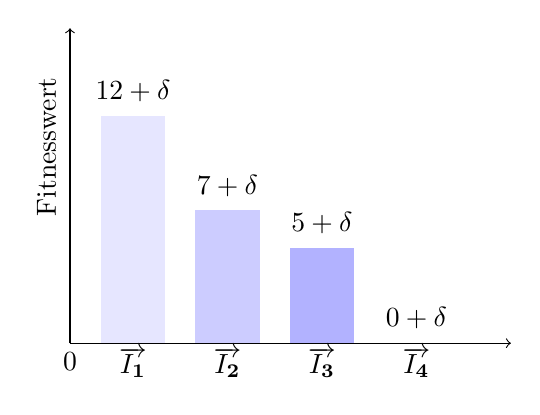
\begin{tikzpicture}[scale=\geneticPlotScale]
            % x-axis label at 0
            \node[below] at (0,0) {0};

            % Bars with numeric labels
            % Bar A
            \filldraw[colorA!50] (0.5,0) rectangle (1.5,\geneticFitnessA*\geneticFitnessScale);
            \node at (1.0,\geneticFitnessA*\geneticFitnessScale+\geneticPlotLabelYoffset) {$\geneticFitnessA+\delta$};

            % Bar B
            \filldraw[colorB!50] (2.0,0) rectangle (3.0,\geneticFitnessB*\geneticFitnessScale);
            \node at (2.5,\geneticFitnessB*\geneticFitnessScale+\geneticPlotLabelYoffset) {$\geneticFitnessB+\delta$};
            % Bar C
            \filldraw[colorC!50] (3.5,0) rectangle (4.5,\geneticFitnessC*\geneticFitnessScale);
            \node at (4.0,\geneticFitnessC*\geneticFitnessScale+\geneticPlotLabelYoffset) {$\geneticFitnessC+\delta$};

            % Bar D
            \filldraw[colorD!50] (5.0,0) rectangle (6.0,\geneticFitnessD*\geneticFitnessScale);
            \node at (5.5,\geneticFitnessD*\geneticFitnessScale+\geneticPlotLabelYoffset) {$\geneticFitnessD+\delta$};
            % Category labels
            \node at (1.0,-0.3) {$\overrightarrow{I_{\mathbf{1}}}$};
            \node at (2.5,-0.3) {$\overrightarrow{I_{\mathbf{2}}}$};
            \node at (4.0,-0.3) {$\overrightarrow{I_{\mathbf{3}}}$};
            \node at (5.5,-0.3) {$\overrightarrow{I_{\mathbf{4}}}$};

            % Axes
            \draw[->] (0,0) -- (7,0); % node[below,]{Individuen};
            \draw[->] (0,0) -- (0,5) node[left, rotate=90, shift={(-0.5,0.3)}]{Fitnesswert};
        \end{tikzpicture}
        \caption{Fitness der Individuen $f(\overrightarrow{I_{\mathbf{i}}})$}
    \end{minipage}
\end{figure}

%\newpage
%\subsubsection{Verbesserte Mutationsstrategie: Relative Mutation}